\documentclass[conference]{IEEEtran}
\IEEEoverridecommandlockouts
\usepackage[T1]{fontenc}
\usepackage{mathptmx}
\usepackage{cite}
\usepackage{amsmath}
\usepackage{graphicx}
\usepackage{booktabs}
\usepackage[hidelinks]{hyperref}
\newcommand{\usd}{\$}
\makeatletter\newcommand{\tabinput}[1]{\@@input #1 }\makeatother
\newcommand{\maxcovstd}{0.004}
\newcommand{\kappafit}{4.0}

\DeclareMathOperator*{\median}{median}

\begin{document}

\title{Conformal Uncertainty Quantification for Physics-Informed American Option Pricing: The Difficulty Score Must Respect Complementarity}

\author{\IEEEauthorblockN{Gaurang Gupta, Arush Gupta, Utkarsh Nigam}
\IEEEauthorblockA{Mukesh Patel School of Technology Management and Engineering (MPSTME)\\
SVKM's NMIMS (Deemed-to-be University), Vile Parle (W), Mumbai 400056, India\\
Email: [GAURANG\_EMAIL] (corresponding author), [ARUSH\_EMAIL], [UTKARSH\_EMAIL]}}

\maketitle

\begin{abstract}
Physics-informed neural networks (PINNs) can price options without labelled prices, but a point price is not a risk number. We study split conformal prediction on top of PINN pricers for European and American puts under geometric Brownian motion, with exact Black-Scholes and 500-step binomial prices as calibration and test labels. Over ten training seeds, the PDE loss cuts the European mean absolute error from \usd 4.42 (a control without the PDE term) to \usd 0.25 and shrinks the 90\% split-conformal band from \usd 19.43 to \usd 0.94. Labelled regressors are more accurate inside their training region, but kernel and polynomial ridge fail outside it. Split conformal reaches nominal marginal coverage for every model, including an American PINN that overprices by \usd 3.13 on average: the bias costs width, not coverage. The raw PDE residual is uninformative for the American put (rank correlation $-0.01$) and widens the band, in part because a positive residual is correct in the exercise region. The complementarity residual $\min(L[u],u-h)$ tracks the error (rank correlation 0.77) and narrows the band from \usd 10.05 to \usd 9.01 at equal coverage. Mondrian buckets give the best worst-bucket coverage (0.86 against 0.71). All labels are synthetic; we claim no market coverage.
\end{abstract}

\begin{IEEEkeywords}
physics-informed neural networks, American options, conformal prediction, uncertainty quantification, no-arbitrage
\end{IEEEkeywords}

\section{Introduction}
A trader who receives a model price also needs to know how far that price may be from the truth. A price without a band is not a risk number. For American options the problem is harder than for European ones, since the early-exercise boundary is unknown and no closed form exists \cite{merton1973theory,hull2022options}. Lattice and simulation methods give accurate references \cite{cox1979option,longstaff2001valuing}, but they do not say how wrong a fast surrogate is at a new point. Learned pricers bring two further issues. Regressors trained on labelled prices need many labels and can break calendar or convexity conditions. PINNs need no labels \cite{raissi2019physics}, but their error is not known in advance.

This paper puts distribution-free conformal bands \cite{vovk2005algorithmic,lei2018distribution} around PINN pricers and asks which difficulty score should scale the band. Our contributions are as follows.
\begin{enumerate}
\item A controlled study of split, residual-normalised and Mondrian conformal prediction on a European PINN (N1), its no-physics control (N0), and an American PINN (N2), over 10 training seeds and 20 calibration splits each.
\item Evidence that the raw PDE residual $|L[u]|$ is a poor difficulty score for the American put, and that the complementarity residual $|\min(L[u],u-h)|$ is a good one. The residual has to follow the structure of the problem.
\item A labelled-baseline comparison and a static-arbitrage check of PINN prices and of interval edges, both reported without repair.
\end{enumerate}
We state the limits at the outset. All labels are synthetic and exact. Our American PINN has a systematic upward bias of \usd 3.13 on a \usd 100 strike. We report no coverage on market quotes.

\section{Related Work}
\emph{Classical pricing.} The Black-Scholes model \cite{black1973pricing} and Merton's rational bounds \cite{merton1973theory} give the European price and the no-arbitrage conditions we test. The binomial lattice of Cox, Ross and Rubinstein \cite{cox1979option} handles early exercise and serves here as the American reference. Barone-Adesi and Whaley \cite{baroneadesi1987efficient} give a fast analytic approximation, and Longstaff and Schwartz \cite{longstaff2001valuing} price American options by least-squares Monte Carlo. Stochastic volatility models \cite{heston1993closed} are usually solved with finite differences, for example ADI schemes \cite{inthout2010adi}. Textbook treatments of parity and early exercise are in \cite{hull2022options}.

\emph{Neural PDE solvers.} PINNs train a network so that a PDE residual, boundary terms and an initial or terminal term are small at sampled points \cite{raissi2019physics}. The Deep Galerkin Method \cite{sirignano2018dgm} follows a similar mesh-free idea and includes an American option example, and the deep BSDE method \cite{han2018solving} targets high-dimensional PDEs. Applied work has used PINNs for Black-Scholes type equations \cite{bai2022application}, for American options \cite{gatta2023meshless} and for the Heston model \cite{hainaut2024option}. To our knowledge, these studies focus on point accuracy rather than on calibrated error bands.

\emph{Labelled learners and shape constraints.} Tree ensembles \cite{ho1995random,breiman2001random} and gradient boosting \cite{friedman2001greedy} are strong tabular regressors. Input-convex networks \cite{amos2017input} build convexity into the architecture, which matches the convexity of option prices in the underlying.

\emph{Conformal prediction.} Conformal prediction gives finite-sample coverage under exchangeability \cite{vovk2005algorithmic}. The inductive or split version uses a held-out calibration set \cite{papadopoulos2002inductive}, and its regression guarantee is analysed in \cite{lei2018distribution}. Normalised scores divide the residual by a local difficulty estimate \cite{papadopoulos2011regression}. Conformalized quantile regression \cite{romano2019conformalized} adapts width through quantile models, and Mondrian conformal regressors \cite{bostrom2020mondrian} calibrate inside categories. A tutorial is given in \cite{angelopoulos2023conformal}.

\emph{Gap.} We found no study that uses the physics residual of a PINN pricer as the conformal difficulty score, and none that asks whether that residual is valid for a free-boundary problem.

\section{Method}
\subsection{Pricing problem}
Let $S$ be the spot, $K$ the strike, $\tau=T-t$ the time to expiry, $r$ the rate, $q$ the dividend yield and $\sigma$ the volatility. We use moneyness $m=S/K$ and the price in strike units $u(m,\tau)=V/K$. The Black-Scholes operator \cite{black1973pricing,merton1973theory} in these coordinates is
\begin{equation}
L[u]=u_\tau-(r-q)\,m\,u_m-\tfrac12\sigma^2m^2u_{mm}+r\,u. \label{eq:op}
\end{equation}
A European put solves $L[u]=0$ with $u(m,0)=h(m)=\max(1-m,0)$, $u(0,\tau)=e^{-r\tau}$ and $u(m_{\max},\tau)=0$. The American put solves the linear complementarity problem (LCP)
\begin{equation}
L[u]\ge0,\qquad u\ge h,\qquad L[u]\,(u-h)=0. \label{eq:lcp}
\end{equation}
In the exercise region $u=h=1-m$, and (\ref{eq:op}) gives $L[h]=r-q\,m$, which equals $r>0$ when $q=0$. So a positive $L[u]$ there is correct, not an error.

\subsection{Networks and losses}
Each PINN is a tanh multilayer perceptron with 4 hidden layers of 64 units on input $(m,\tau)$. We use tanh because the residual needs $u_{mm}$, and the second derivative of a ReLU network is zero almost everywhere. Derivatives come from automatic differentiation in PyTorch \cite{paszke2019pytorch}. Let $\overline{(\cdot)}$ denote a mean over points resampled every epoch: 3000 interior points on $[0,3]\times[0,1]$, 400 terminal points (half of them near $m=1$) and 200 boundary points. The European loss is
\begin{equation}
\mathcal L_{\mathrm{E}}=\lambda_{p}\,\overline{L[u]^2}+3\,\overline{(u-h)^2}_{\tau=0}+\overline{(u-g)^2}_{\partial}, \label{eq:le}
\end{equation}
where $g$ is the boundary value. N1 uses $\lambda_p=1$. N0 uses $\lambda_p=0$, so it fits only the payoff and the edges; it is the control. The American loss N2 replaces the PDE term with three LCP penalties, each with weight 1,
\begin{equation}
\overline{\mathrm{relu}(-L[u])^2}+\overline{\mathrm{relu}(h-u)^2}+\overline{(L[u](u-h))^2}, \label{eq:la}
\end{equation}
plus the same terminal and boundary terms. All runs use fixed weights. Training uses Adam with learning rate $2\times10^{-3}$, halved every 2000 of 6000 epochs. The PINNs see no labelled price.

\subsection{Labelled baselines}
Table~\ref{tab:base} lists ten labelled regressors from an earlier project run. They learn $(m,\tau)\mapsto u$ from 500-step binomial labels \cite{cox1979option}. The four classical models use scikit-learn \cite{pedregosa2011scikit} and the six networks use PyTorch.

\subsection{Conformal intervals}
Let $\hat u$ be a PINN prediction and $R(m,\tau)$ a signed residual. On $n$ calibration points with exact labels we compute
\begin{equation}
s_i=\frac{|u_i-\hat u_i|}{1+\kappa|R_i|},\qquad \kappa=\frac{1}{\median_i|R_i|}. \label{eq:score}
\end{equation}
With $\kappa=0$ this is split conformal \cite{papadopoulos2002inductive}; with $\kappa>0$ it is a normalised score \cite{papadopoulos2011regression}. Let $q$ be the $k$-th smallest score with
\begin{equation}
k=\lceil (n+1)(1-\alpha)\rceil , \label{eq:k}
\end{equation}
which is the finite-sample quantile of split conformal \cite{lei2018distribution}. The band in dollars at a test point is
\begin{equation}
\big[K\hat u-Kq(1+\kappa|R|),\;K\hat u+Kq(1+\kappa|R|)\big]. \label{eq:band}
\end{equation}
If calibration and test points are exchangeable, the band covers the true price with probability at least $1-\alpha$ \cite{lei2018distribution}. We compare four scores: split ($\kappa=0$); normalised with $R=L[u]$; for N2 only, normalised with the LCP residual $R=\min(L[u],u-h)$, which is zero exactly when (\ref{eq:lcp}) holds; and Mondrian \cite{bostrom2020mondrian}, which computes $q$ separately in six buckets, $m<0.9$, $0.9\le m\le1.1$, $m>1.1$, each crossed with $\tau<0.4$ and $\tau\ge0.4$.

\section{Experiments}
\subsection{Setup}
We fix $r=0.03$, $q=0$, $\sigma=0.2$ and $K=100$. We train N0, N1 and N2 with seeds 0 to 9 (30 runs). For each seed we draw 4000 points with $m\sim U[0.6,1.4]$ and $\tau\sim U[0.05,1]$ and label them with the Black-Scholes formula (European) or the 500-step binomial tree (American). For each of 20 random splits, the first $n_{\mathrm{cal}}=800$ points calibrate and the next 2000 test; $n_{\mathrm{cal}}=400$ gave the same picture. We use $\alpha\in\{0.10,0.05\}$. We average over splits within a seed, then over seeds. ``Worst bucket'' is the lowest of the six bucket coverages in a split, averaged the same way. The protocol was written before any coverage was computed and was not changed. All runs used CPU only, on an 8-vCPU Intel Xeon cloud machine with one thread per run and 8 runs in parallel. The 30 trainings took 12 min 24 s in total; one run took 157 s (N0), 167 s (N1) and 229 s (N2) on average. All conformal evaluations took 62 s. Numerical code used NumPy \cite{harris2020array}.

\begin{table}[t]
\caption{Labelled baselines for the American put (MAE in \usd, $K=100$). Earlier project run on a separate $25\times9$ test grid, mean of 2 seeds. ``Box'': labels only for $m\in[0.85,1.15]$, $\tau\le0.5$, scored inside and outside the box. Violation rates are finite-difference checks on the full-label grid at 3000 labels.}
\label{tab:base}
\centering\footnotesize\setlength{\tabcolsep}{2.6pt}
\begin{tabular}{lrrrrrr}
\toprule
 & \multicolumn{2}{c}{Full labels} & \multicolumn{2}{c}{Box, 3000} & \multicolumn{2}{c}{Viol. rate}\\
Model & $n{=}50$ & 3000 & in & out & convex & calendar\\
\midrule
\tabinput{tables/table1_baselines.tex}
\bottomrule
\end{tabular}
\end{table}

\subsection{Labelled baselines}
Table~\ref{tab:base} confirms that labels win inside the labelled region. With 3000 labels, kernel ridge reaches \usd 0.005 against \usd 2.313 for the N2 PINN of that run, and all ten labelled models beat the PINN; with 50 labels, nine of ten do. When labels cover only a strip near the money, kernel ridge and polynomial ridge reach \usd 67.06 and \usd 142.81 outside it, while the PINN stays at \usd 2.55, close to its full-grid error. The PINN also has no calendar violations. The Black-Scholes-embedded network is the best model outside the box (\usd 0.13), since it builds in the pricing formula.

\begin{table}[t]
\caption{PINN point accuracy on the calibration/test pools (mean of 10 seeds, \usd). Bias is the mean signed error; ``Above'' is the share of points priced above the reference; $\rho$ is the Spearman rank correlation of the absolute residual with the absolute error.}
\label{tab:point}
\centering\footnotesize\setlength{\tabcolsep}{2.4pt}
\begin{tabular}{lrrrrrrr}
\toprule
Model & MAE & Max & Bias & Above & $\rho_{|L|}$ & $\rho_{\mathrm{LCP}}$ & Train s\\
\midrule
\tabinput{tables/table2_point.tex}
\bottomrule
\end{tabular}
\end{table}

\subsection{Point accuracy and the residual signal}
Table~\ref{tab:point} shows that the PDE term matters. N1 reaches an MAE of \usd 0.25, while the N0 control has \usd 4.42. N2 has an MAE of \usd 3.13 that is almost all bias: it prices 99.6\% of points above the binomial reference. The residuals behave differently by model. For N0 the raw residual $|L[u]|$ tracks the error ($\rho=0.56$), because N0 never fits the PDE. For N1 it is weak ($\rho=0.15$). For N2 it carries no signal ($\rho=-0.01$), while the LCP residual has $\rho=0.77$. Fig.~\ref{fig:resid} shows the pattern for one seed. The raw residual stays in a narrow band (median 0.057) whatever the price error. One reason is structural: in the exercise region the exact solution has $L[u]=r$, so a large $|L[u]|$ there is not an error. The LCP residual removes this part and rises with the error.

\begin{figure}[t]
\centering
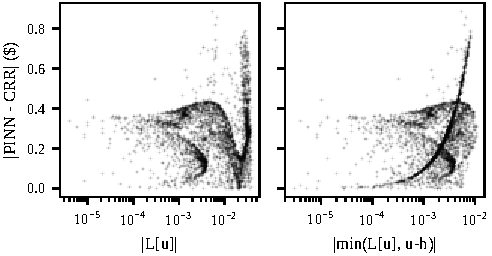
\includegraphics[width=\columnwidth]{figures/fig_p2_residual_vs_error.pdf}
\caption{N2, seed 0, 4000 pool points. Absolute price error against the raw residual $|L[u]|$ (left) and the LCP residual (right). The raw residual stays in a narrow band for any error; the LCP residual rises with the error.}
\label{fig:resid}
\end{figure}

\begin{table}[t]
\caption{Conformal bands, $n_{\mathrm{cal}}=800$, $n_{\mathrm{test}}=2000$, mean over 10 seeds $\times$ 20 splits. Width in \usd. Seed-to-seed std of coverage is at most \maxcovstd{}.}
\label{tab:conf}
\centering\footnotesize\setlength{\tabcolsep}{2.6pt}
\begin{tabular}{llrrrrrr}
\toprule
 & & \multicolumn{3}{c}{$\alpha=0.10$} & \multicolumn{3}{c}{$\alpha=0.05$}\\
Model & Score & Cov. & Width & Worst & Cov. & Width & Worst\\
\midrule
\tabinput{tables/table3_conformal.tex}
\bottomrule
\end{tabular}
\end{table}

\subsection{Conformal bands on PINN pricers}
Table~\ref{tab:conf} gives the main result. Marginal coverage is at its nominal level for every model and score, within 0.005. This holds for N2 too, despite its bias. The finite-sample guarantee does its job; the bias shows up as width. The PDE term shrinks the split band from \usd 19.43 (N0) to \usd 0.94 (N1) at $\alpha=0.10$, about 20 times. The choice of difficulty score matters. Normalising by $|L[u]|$ widens the N1 band (\usd 1.18 against \usd 0.94) and the N2 band (\usd 11.89 against \usd 10.05). It helps only N0, whose residual is large where it fails. For N2, the LCP residual gives \usd 9.01 against \usd 10.05 at the same coverage, but its worst bucket (0.71) is no better than split. Mondrian gives the narrowest bands and the best worst-bucket coverage (0.86 against 0.71 for split on N2). Fig.~\ref{fig:bucket} shows that split over-covers short tenors and under-covers deep in-the-money long tenors (0.71), while Mondrian keeps each bucket between 0.902 and 0.910 on average. Fig.~\ref{fig:slice} shows the bands on one slice: they contain the reference, but they are wide because the PINN sits above it.

\begin{figure}[t]
\centering
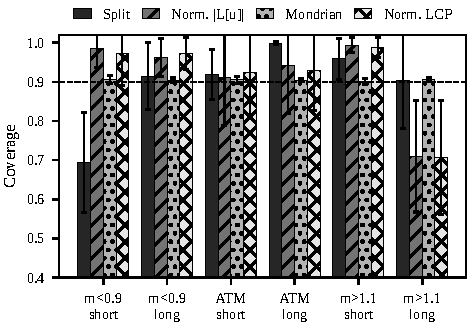
\includegraphics[width=\columnwidth]{figures/fig_p2_bucket_coverage_a10.pdf}
\caption{N2, $\alpha=0.10$, $n_{\mathrm{cal}}=800$: coverage per moneyness and tenor bucket (short: $\tau<0.4$), mean and std over 10 seeds. Dashed line: target 0.90. Only Mondrian is close to target in every bucket.}
\label{fig:bucket}
\end{figure}

\begin{figure}[t]
\centering
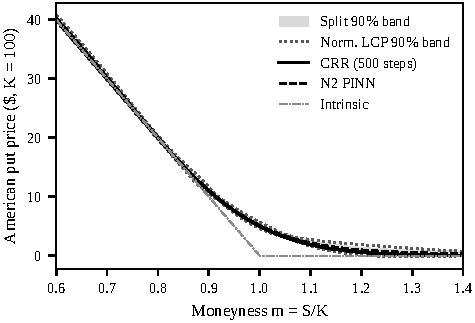
\includegraphics[width=\columnwidth]{figures/fig_p2_interval_slice_tau050.pdf}
\caption{American put at $\tau=0.5$, seed 0, $\alpha=0.10$. The split band (grey) and the LCP-normalised band (dotted) both contain the binomial price; the PINN lies above it, so the bands are wide and the lower edges fall below zero out of the money.}
\label{fig:slice}
\end{figure}

\subsection{Synthetic heteroscedastic check}
To isolate the score, we reuse a synthetic set with a known mean, noise standard deviation $0.01+0.12|m-1|$, difficulty $|m-1|$, $n_{\mathrm{cal}}=800$, $n_{\mathrm{test}}=2500$ and 50 seeds (Table~\ref{tab:p3}). Normalisation narrows the band (0.127 against 0.145 at $\alpha=0.10$) and raises coverage far from the money from 0.813 to 0.854. The fitted $\kappa$ is \kappafit{}, while the true ratio of slope to intercept is 12, so the adaptation is only partial. With homoscedastic noise, split coverage is 0.903 ($\alpha=0.10$) and 0.953 ($\alpha=0.05$).

\begin{table}[t]
\caption{Synthetic heteroscedastic data, 50 seeds. Width in $u$ units. Near: $|m-1|\le0.25$; far: $|m-1|>0.25$.}
\label{tab:p3}
\centering\footnotesize\setlength{\tabcolsep}{3.5pt}
\begin{tabular}{llrrrr}
\toprule
$\alpha$ & Score & Cov. & Width & Near & Far\\
\midrule
\tabinput{tables/table4_p3.tex}
\bottomrule
\end{tabular}
\end{table}

\subsection{Static arbitrage of prices and band edges}
We run the project's arbitrage checker on a put chain with $S=100$, strikes 60 to 140 in steps of 2.5 and ten expiries from 0.1 to 1 year, with tolerance $10^{-6}$ (Table~\ref{tab:p4}). Bands come from split 0, $n_{\mathrm{cal}}=800$, $\alpha=0.10$. The PINN prices break strike convexity in 12\% (N1) and 26\% (N2) of checkable triples. A constant split band keeps the convexity and calendar rates of the point price, since it only adds a term linear in $K$, but its lower edge raises monotonicity violations from 0.010 to 0.059. Bands of varying width add violations. About a third of lower edges are negative. The calendar check is not a valid condition for European puts: the exact Black-Scholes chain fails it in 27\% of cases. We apply no repair.

\begin{table}[t]
\caption{Static-arbitrage violation rates on a synthetic put chain (mean of 10 seeds). Put-call parity is not applicable to a put-only chain.}
\label{tab:p4}
\centering\footnotesize\setlength{\tabcolsep}{3pt}
\begin{tabular}{lrrrr}
\toprule
Series & Monot. & Convex & Calendar & Price${<}0$\\
\midrule
\tabinput{tables/table5_p4.tex}
\bottomrule
\end{tabular}
\end{table}

\section{Discussion}
\emph{Why keep the PINN if it loses on MAE?} It needs no labels, and it degrades gently outside any labelled region, where kernel and polynomial ridge fail (Table~\ref{tab:base}). It also exposes a residual for free. With a conformal layer, even a biased PINN gives bands with valid marginal coverage. The cost of the bias is width, so a better PINN gives narrower bands at once, as N1 against N0 shows.

\emph{Which residual?} The residual should measure distance from the conditions that define the solution. For a European option that is $L[u]=0$. For an American option it is the LCP (\ref{eq:lcp}), and $|L[u]|$ is not zero at the true solution in the exercise region. The LCP residual fixes this and is a much better error proxy. Still, Mondrian buckets beat it on conditional coverage here, so the two ideas can be combined in future work.

\emph{The N2 bias.} N2 is above the reference almost everywhere, also deep out of the money where early exercise hardly matters. We did not tune N2 after seeing these numbers. Candidate causes are the fixed loss weights and the boundary at $m=0$, where our code imposes the European value $e^{-r\tau}$ rather than the American value 1. We have not tested these causes.

\emph{What the data cannot show.} The project holds one Yahoo Finance snapshot of 4054 quotes from 13 Aug 2026 for SPX, NDX, NVDA and AAPL. One snapshot cannot support a time-ordered calibration and test split, so we report no market coverage. Real quotes also carry bid-ask noise and are not exchangeable across dates.

\section{Conclusion}
We placed split, normalised and Mondrian conformal bands on European and American PINN pricers. Marginal coverage held for every model, including a biased American PINN. The PDE loss shrank the European band about 20 times. Labelled regressors remain more accurate in-sample.

The difficulty score must match the problem. The raw PDE residual is a poor score for the American put, and the complementarity residual is a good one. Future work will fix the N2 bias, build a dated market panel for real coverage tests, project band edges onto arbitrage-free prices, and put a band on the exercise boundary $S^*(\tau)$.

\section*{Acknowledgment}
The authors thank Dr. Manish Kumar Tiwari for guidance. AI-use disclosure: an AI assistant (Grok Bot) wrote the experiment scripts, drew the figures and drafted the text of all sections; the authors reviewed, revised and verified all content and take responsibility for it.

\bibliographystyle{IEEEtran}
\bibliography{references}

\end{document}
